\documentclass[10pt,twocolumn]{article}
\usepackage[a4paper,top=18mm,bottom=20mm,left=16mm,right=16mm,columnsep=7mm]{geometry}
\usepackage[T1]{fontenc}
\usepackage{lmodern}
\usepackage{microtype}
\usepackage{amsmath,amssymb,mathtools}
\usepackage{graphicx}
\usepackage{booktabs,tabularx,array}
\usepackage[table]{xcolor}
\usepackage{caption}
\usepackage{float}
\usepackage{enumitem}
\usepackage[hidelinks]{hyperref}
\usepackage{fancyhdr}

\definecolor{navy}{HTML}{13233F}
\definecolor{blue}{HTML}{2563A6}
\definecolor{cyan}{HTML}{168F91}
\definecolor{coral}{HTML}{D85E52}
\definecolor{pale}{HTML}{EEF4F8}
\definecolor{muted}{HTML}{5D6975}
\hypersetup{colorlinks=true,linkcolor=blue,citecolor=blue,urlcolor=blue}
\captionsetup{font=small,labelfont={bf,color=navy}}
\setlength{\parindent}{1em}
\setlength{\parskip}{0pt}
\setlength{\emergencystretch}{2em}
\setlist{nosep,leftmargin=*}
\pagestyle{fancy}
\fancyhf{}
\fancyhead[L]{\footnotesize\color{muted}Exploratory Stage C report}
\fancyhead[R]{\footnotesize\color{muted}Compact Titans DNA model}
\fancyfoot[C]{\thepage}
\renewcommand{\headrulewidth}{0.3pt}
\newcommand{\code}[1]{\texttt{#1}}
\newcommand{\R}{\mathbb{R}}
\newcommand{\norm}[1]{\left\lVert#1\right\rVert}
\newcommand{\had}{\odot}

\graphicspath{{../../artifacts/stage_c_c16_scientific_package/figures/}}

\begin{document}
\twocolumn[
\begin{center}
{\color{navy}\rule{\textwidth}{1.2pt}}\par\vspace{7pt}
{\LARGE\bfseries\color{navy} DNA generation by a compact Titan neural-memory model shows promising genetic features but incomplete genome organization\par}
\vspace{7pt}
{\large Stage C c16 exploratory study report\par}
\vspace{4pt}
{\small SeqTrainer Titans programme \textbullet{} 31 July 2026 \textbullet{} exploratory, not peer reviewed\par}
\vspace{7pt}
\begin{minipage}{0.94\textwidth}
\small
\textbf{Abstract.}
Neural long-term memory is an appealing mechanism for modelling genomes, whose constraints span nucleotides, motifs, genes and chromosome-scale organization. We evaluated a compact, 2.52-million-parameter, four-block Memory-as-Context model trained on 5 million valid bases of \textit{Escherichia coli}-related sequence. The implementation couples causal attention to a stream-local, two-layer residual neural memory updated by gradients of a key--value association loss. Held-out next-token performance reached 1.9828 bits per base (BPB). In a controlled association probe, adaptive memory reduced reconstruction error by 9.60--11.31\% across the four blocks. Conditional generations preserved near-reference nucleotide entropy and sequence diversity, and an unrestricted temperature-0.8 decoder recovered the reference median gene-call rate (8.14 per 10 kb). However, generated GC fraction was low (0.467 versus 0.514), 6-mer divergence was substantial (Jensen--Shannon divergence 0.326), coding density was reduced (0.330 versus 0.494), predicted genes were shorter, and intergenic intervals were much longer. Memory and embedding principal-component analyses were technically successful but used only one accession and cannot establish taxonomic organization; memory PC1 was more correlated with stream position than GC content. These results show stable learning, active associative memory and non-trivial local genetic statistics, but do not demonstrate functional genes, coherent genomes, biological viability, adaptive-memory superiority or taxonomic representation. Matched controls and broader held-out panels are required before scaling claims.
\end{minipage}
\vspace{8pt}
{\color{navy}\rule{\textwidth}{0.6pt}}
\end{center}
\vspace{4pt}
]

\section*{Motivation and scope}
Genome language models must learn regularities at several scales. Short-range composition can produce plausible-looking DNA without reconstructing genes or chromosome organization; conversely, a low token loss does not by itself show that an explicit memory mechanism caused the gain. Titans introduces a train-time-learned neural memory whose \emph{fast weights} change while a sequence is processed, potentially supplying state beyond the local attention context \cite{behrouz2025titans}. The present study asks a deliberately narrower question: after a small exploratory training run, does the c16 model show enough stable learning, memory activity and generative structure to justify a larger controlled study?

This is an evidence-gating experiment, not a claim of a genome generator. The model was trained only on a restricted \textit{E. coli}-related corpus, the generative evaluation was small, predicted open reading frames (ORFs) were produced by a gene caller rather than laboratory validation, and no matched no-memory model was trained at the same 5-million-base scale.

\section*{Dataset construction and relation to the parent corpus}
The parent resource, \nolinkurl{bacteria_titan_v1_ecoli_related_15gbp}, was designed as a nominal 15-Gbp bacterial corpus from NCBI assemblies annotated with GTDB R220 metadata \cite{gtdbr220}. Selection expanded outwards from \textit{E. coli} to other \textit{Escherichia}, Enterobacteriaceae and Enterobacterales, with nominal base budgets of 35\%, 15\%, 30\% and 20\%, respectively. Assemblies were required to have estimated completeness of at least 90\%, contamination no greater than 5\%, and genome size between 0.5 and 12 Mbp. Within those constraints, the builder preferred representatives and higher-quality assemblies while rotating through diversity groups. Thus the parent corpus is \textit{E. coli}-centred but is not an \textit{E. coli}-only collection.

Stage C derived an ordered-stream dataset from the frozen parent accession manifest and cached NCBI FASTA archives. Assembly accessions were canonicalized before splitting. Within \textit{E. coli}, pairwise average nucleotide identity (ANI) estimated by skani \cite{shaw2023skani} was converted into deterministic 99\%-ANI single-linkage groups; outside \textit{E. coli}, GTDB species clusters supplied the grouping. Complete groups, rather than fragments or token windows, were assigned to train, validation and test in approximate 90:5:5 proportions, weighted by manifest genome size and stratified by sampling scope. This prevents the same accession or declared clade group from crossing splits. Each contig or replicon then became an independent ordered memory stream, was normalized to uppercase DNA, and was encoded into non-overlapping 6-mers. Token IDs and each token's represented-base length were stored in checksummed, memory-mapped shards; 32-token causal segments were created lazily without crossing contig boundaries.

The c16 checkpoint did not consume this entire hierarchy. It processed 5,000,000 valid target bases from the train split under a deterministic, seed-shuffled stream-to-completion scheduler. This is only 0.033\% of the parent's nominal 15-Gbp design target, and the 15-Gbp denominator is a corpus target rather than an audited c16 exposure denominator. Moreover, the c16 evidence package did not export taxon-by-taxon counts for the exact 5-million-base trajectory. The exposure therefore cannot be assumed to be a uniform or clade-balanced miniature of the parent corpus. Generation was evaluated separately on held-out sequences labelled \textit{E. coli}; those prompts were excluded from fitting by the group-level split.

\begin{figure*}[t]
\centering
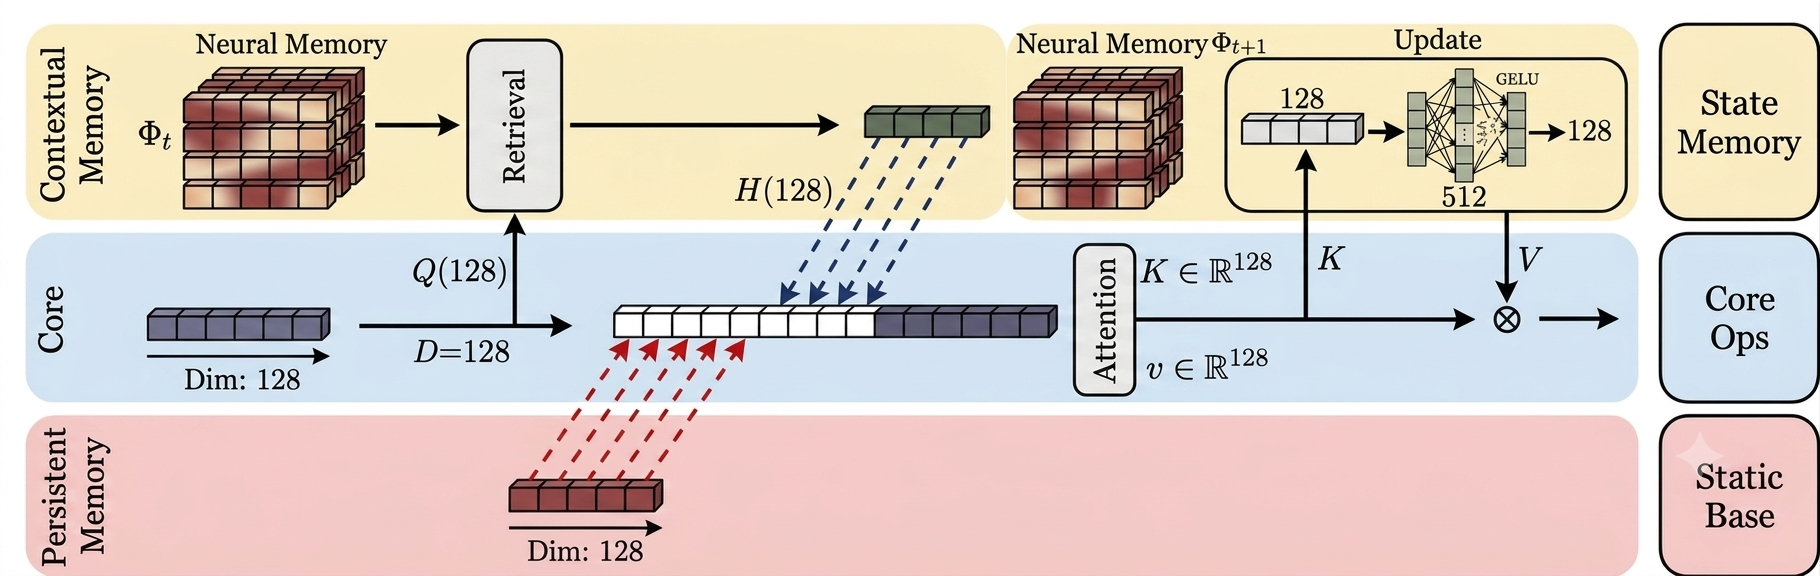
\includegraphics[width=0.96\textwidth]{figure_1_model_architecture.png}
\caption{\textbf{Memory-focused schematic of the evaluated architecture.} The diagram separates persistent learned context, causal core operations and stream-local neural memory, emphasizing retrieval followed by a key--value-driven fast-weight update. It is a conceptual view rather than a complete layer inventory: the evaluated model embeds non-overlapping 6-mer tokens in 128 dimensions and stacks four causal Memory-as-Context blocks. The exact read-before-write timing, $[P;H;Z]$ layout, projections and recurrence are specified below and take precedence over pictorial shorthand.}
\label{fig:architecture}
\end{figure*}

\section*{Model and mathematical specification}
\subsection*{Tokens, segments and slow versus fast state}
Let the nucleotide string be partitioned into non-overlapping 6-mers. A token has vocabulary index $a_t\in\{1,\ldots,V\}$ at global token position $t$, with vocabulary size $V=4{,}103$. The learned embedding $E\in\R^{V\times d}$ maps $a_t$ to $x_t=E[a_t]\in\R^d$, where the model width is $d=128$. Processing occurs in segments of $C=32$ tokens. We use $n$ for a segment and $i\in\{1,\ldots,C\}$ for a position inside that segment; this distinction prevents the paper's generic time subscript from being confused with the implementation's segment boundary.

The four stacked MAC blocks have slow parameters, collectively denoted $\omega$, learned by the outer language-model objective. Each block and logical sequence stream also has fast memory parameters $\phi_{n,i}$ and a surprise-momentum state $S_{n,i}$. Fast state is reset between independent streams. It is differentiable within the configured truncation horizon of three segments; it is not a free-standing database and is not shared between genomes.

\subsection*{Read projections and neural memory}
For one block, let $z_{n,i}\in\R^d$ denote its input representation at position $i$. The implementation first applies learned linear maps $W_Q,W_K,W_V\in\R^{d\times d}$ and then separate causal depth-wise convolutions of kernel width four. Writing $\mathcal C_Q,\mathcal C_K,\mathcal C_V$ for these convolution operators,
\begin{align}
q_{n,i}&=\operatorname{unit}\!\left(\mathcal C_Q(W_Qz_{n,i})\right),\label{eq:q}\\
k_{n,i}&=\operatorname{unit}\!\left(\mathcal C_K(W_Ky_{n,i})\right),\label{eq:k}\\
v_{n,i}&=\mathcal C_V(W_Vy_{n,i}),\label{eq:v}
\end{align}
where $q_{n,i}$ is the read query, $k_{n,i}$ and $v_{n,i}$ are the write key and target value, and $y_{n,i}$ is the block's post-attention representation. The operation $\operatorname{unit}(u)=u/\max(\norm{u}_2,\epsilon)$ L2-normalizes queries and keys, where $u\in\R^d$ is any projected vector and $\epsilon$ is the smallest safe positive value for the numerical data type. Values are not normalized. Convolution history is stream-local.

The neural memory is a two-layer, four-times-expanded residual multilayer perceptron (MLP):
\begin{equation}
M_{\phi}(u)=u+\operatorname{LN}\!\left[W_o\operatorname{GELU}(W_i u+b_i)+b_o\right].\label{eq:mlp}
\end{equation}
Here $M_{\phi}:\R^d\rightarrow\R^d$ is the memory function; $u\in\R^d$ is its input; $W_i\in\R^{4d\times d}$ and $b_i\in\R^{4d}$ form the expansion layer; $W_o\in\R^{d\times4d}$ and $b_o\in\R^d$ form the output layer; $\operatorname{GELU}$ is the Gaussian error linear unit; $\operatorname{LN}$ is layer normalization; and $\phi=\{W_i,b_i,W_o,b_o,$ layer-normalization scale and bias$\}$ is the complete fast-parameter set. Retrieval is
\begin{equation}
h_{n,i}=M_{\phi_{n,0}}(q_{n,i}),\label{eq:retrieve}
\end{equation}
where $h_{n,i}\in\R^d$ is the retrieved vector and $\phi_{n,0}$ is the incoming fast state. All $C=32$ retrievals in a segment use this same incoming state; writes occur after the attention calculation.

\subsection*{Causal Memory-as-Context integration}
Let $P\in\R^{p\times d}$ be a learned bank of $p=4$ persistent tokens, $H_n=[h_{n,1},\ldots,h_{n,C}]$ the retrieval matrix and $Z_n=[z_{n,1},\ldots,z_{n,C}]$ the input matrix. The implementation packs
\begin{equation}
L_n=[P;H_n;Z_n]\in\R^{(p+2C)\times d},\label{eq:layout}
\end{equation}
where $[\,;\,]$ means row-wise concatenation. Multi-head self-attention has four heads and a block-causal mask: the query associated with position $i$ may attend to all persistent tokens and to retrieval/input positions $1{:}i$, but never to a future position $j>i$. The selected sequence output receives a residual connection and layer normalization to give $y_{n,i}$. Four such blocks are stacked.

This explicit $[P;H;Z]$ layout is an implementation choice that preserves the intended causal read-as-context operation. It should not be mistaken for a literal reproduction of every concatenation order printed in the Titans exposition.

\subsection*{Associative objective and surprise recurrence}
At write position $i$, the implemented inner objective is
\begin{align}
\ell_{n,i}(\phi)&=\frac{1}{2}\norm{M_{\phi}(k_{n,i})-v_{n,i}}_2^2,\nonumber\\
g_{n,i,r}&=\nabla_{\phi_r}\ell_{n,i}(\phi_{n,i-1}).\label{eq:assoc}
\end{align}
where $\ell_{n,i}\in\R$ is associative reconstruction loss, $g_{n,i,r}$ is its gradient for fast-parameter tensor $r$, and $\phi_r$ denotes that tensor. The squared error is summed over the $d$ output channels. The subscript $r$ ranges over the six fast tensors in Eq.~\eqref{eq:mlp}.

The per-tensor update is
\begin{align}
S_{n,i,r}&=\eta_{n,i,r}\had S_{n,i-1,r}-\theta_{n,i,r}\had g_{n,i,r},\label{eq:momentum}\\
\phi_{n,i,r}&=(1-\alpha_{n,i,r})\had\phi_{n,i-1,r}+S_{n,i,r}.\label{eq:forget}
\end{align}
Here $S_{n,i,r}$ is accumulated surprise momentum; $\eta_{n,i,r}\in(0,1)$ retains past surprise; $\theta_{n,i,r}\in(0,1)$ scales the momentary gradient write; $\alpha_{n,i,r}\in(0,1)$ is the fraction of the old fast weight forgotten; $1$ is a tensor of ones with compatible shape; and $\had$ denotes element-wise multiplication with broadcasting. Learned sigmoid gate heads produce values per MLP layer and output channel, which are broadcast across each parameter's input dimension. Initialization was $\alpha=0.001$, $\eta=0.9$ and $\theta=0.001$. For the c16 \code{paper\_exact} policy, neither surprise-norm clipping nor RMS gradient conditioning was enabled.

After position $C$, $(\phi_{n,C},S_{n,C})$ becomes the incoming state $(\phi_{n+1,0},S_{n+1,0})$ for the next segment. The word ``momentum'' therefore refers to momentum in the inner associative-gradient process, not the optimizer used for slow parameters.

\paragraph{Factor convention relative to the paper.}
The Titans paper prints $\norm{M(k)-v}_2^2$ without the factor $1/2$ \cite{behrouz2025titans}. This implementation uses Eq.~\eqref{eq:assoc}, so its gradient is exactly one half of the gradient of the printed objective at the same $\phi,k,v$. Both losses have the same minimizers, but the effective write magnitude is rescaled and must be interpreted jointly with $\theta$. Thus ``paper exact'' here describes the unconditioned sequential recurrence and deep-memory policy, not identity of this loss prefactor.

The operational path is therefore specified directly by the equations: retrieval uses Eq.~\eqref{eq:retrieve}, momentary surprise is the associative gradient in Eq.~\eqref{eq:assoc}, past and momentary surprise combine through Eq.~\eqref{eq:momentum}, and Eq.~\eqref{eq:forget} applies forgetting while committing the new fast state.

\subsection*{Outer objective and bits per base}
For target token $a_t$ and preceding context $a_{<t}$, the slow model assigns probability $p_{\omega}(a_t\mid a_{<t})$. The outer negative log-likelihood is
\begin{equation}
\mathcal L_{\mathrm{LM}}=-\sum_{t\in\mathcal T}\log p_{\omega}(a_t\mid a_{<t}),\qquad
\mathrm{BPB}=\frac{\mathcal L_{\mathrm{LM}}}{N_b\log 2}.\label{eq:bpb}
\end{equation}
Here $\mathcal T$ is the set of valid predicted token positions, $\omega$ contains all learned slow parameters (including initial memory meta-parameters and gate networks), $N_b$ is the number of represented valid nucleotide bases, and $\log$ is the natural logarithm. BPB converts total natural-log loss to binary information per nucleotide. A uniform independent A/C/G/T baseline is 2 BPB; values below 2 indicate predictive signal, but not necessarily biological function.

\section*{Generation and analysis methods}
\subsection*{Conditional decoding}
Generation transformed next-token logits $r_j\in\R$ for vocabulary item $j$ into probabilities
\begin{equation}
\pi_j(T)=\frac{\exp(r_j/T)}{\sum_{m\in\mathcal A}\exp(r_m/T)},\label{eq:softmax}
\end{equation}
where $T>0$ is temperature, $\mathcal A$ is the currently allowed candidate set, $m$ indexes candidates in that set and $\pi_j(T)$ is the sampling probability. Top-$k$ retains only the $k$ largest-logit tokens. Nucleus sampling retains the smallest probability-ranked set whose cumulative mass reaches $p$; here $p\in(0,1]$ is the nucleus threshold, not a model parameter. ``No-$k$'' means no top-$k$ restriction. Nine decoding policies varied $T\in\{0.6,0.8,1.0,1.1\}$, $k\in\{128,512,1024,\text{none}\}$ and $p\in\{0.95,0.99,1.0\}$ on the same checkpoint.

\subsection*{Sequence metrics}
GC fraction is the proportion of generated nucleotides that are G or C. Nucleotide entropy is $H=-\sum_{b\in\{A,C,G,T\}}f_b\log_2 f_b$, where $f_b$ is the observed frequency of base $b$ and $H$ is measured in bits; 2 bits is the maximum for four equally frequent bases. Aligned and overlapping diversity quantify pairwise sequence disagreement at fixed positions and overlapping windows, respectively. Homopolymer length records the longest same-base run.

For $q$-mer frequency distributions $P_q$ and $Q_q$ from reference and generated sequences, Jensen--Shannon divergence is
\begin{align}
R_q&=\tfrac12(P_q+Q_q),\nonumber\\
\operatorname{JSD}(P_q,Q_q)&=\tfrac12\operatorname{KL}(P_q\Vert R_q)
 +\tfrac12\operatorname{KL}(Q_q\Vert R_q).\label{eq:jsd}
\end{align}
where $q\in\{1,\ldots,6\}$ is word length, $R_q$ is the mixture distribution, and $\operatorname{KL}$ is Kullback--Leibler divergence using the same log base for every comparison. JSD is zero only for identical distributions; increasing values indicate increasing compositional mismatch.

\subsection*{Prodigal gene-structure diagnostics}
Prodigal is an ab initio prokaryotic protein-coding gene finder, not a homology search or a functional assay \cite{hyatt2010prodigal}. It scores candidate open reading frames on both strands using sequence-derived coding statistics, including frame-dependent hexamer composition, together with start/stop-codon structure and translation-initiation evidence such as ribosome-binding-site motifs. Dynamic programming then selects a mutually compatible, high-scoring set of coding sequence (CDS) calls. Because the generated and reference continuations were short fragments rather than complete chromosomes, both FASTA collections were analysed with the same Prodigal metagenomic policy (\code{-p meta}). That policy selects among pre-trained organism models instead of estimating one genome-specific model from each fragment. Keeping the invocation identical makes generated/reference differences interpretable as sequence differences rather than gene-caller settings.

CDS coordinates from Prodigal's GFF output were used to calculate calls per 10 kb, median called-gene length and the fraction of each sequence covered by the union of CDS intervals (predicted coding density). Gaps between merged CDS intervals, including terminal gaps, defined the reported intergenic lengths. The complete-call fraction was also retained from Prodigal's partial-call annotation. Separately, the transparent six-frame ORF scan counted start-to-stop intervals of at least 90 bp; it was not treated as a second gene caller.

These diagnostics probe whether sampled output contains the local statistical cues that a microbial gene finder recognizes and whether those cues are arranged over longer spans. They do not observe hidden embeddings or fast-memory weights directly. Consequently, a positive Prodigal call supports only the statement that the model's conditional output distribution contains some coding-like sequence evidence. It cannot identify which internal representation produced that evidence, demonstrate that neural memory caused it, or establish transcription, translation, protein function or viability.

\subsection*{Memory probe and principal components}
The controlled association probe compares key--value reconstruction before and after an adaptive memory update. Percentage improvement is $100(\ell_{\mathrm{before}}-\ell_{\mathrm{after}})/\ell_{\mathrm{before}}$, where both losses use Eq.~\eqref{eq:assoc}. A positive value shows that the update stored the tested association; it does not show that this storage improves held-out language modelling.

For PCA, a feature matrix $X\in\R^{n_s\times d_f}$ was centered over its $n_s$ observations and $d_f$ features. Eigenvectors $u_1,u_2\in\R^{d_f}$ of the sample covariance define scores $c_{j,r}=X_j u_r$ for observation $j$ and component $r\in\{1,2\}$. Explained-variance fraction is the eigenvalue for component $r$ divided by the sum of all eigenvalues. Memory PCA used $n_s=206$ segment observations; embedding PCA used eight stream-mean observations. The feature dimension $d_f$ is specific to each exported representation and is distinct from model width $d$.

\section*{Results}
\subsection*{The model learned a modest held-out signal}
Held-out performance reached 1.9828 BPB, 0.0172 BPB below the uniform four-base reference. This confirms finite, non-random predictive learning under the evaluated split and tokenizer. The margin is small: it does not establish useful genome modelling on its own and cannot identify which component caused the gain.

The adaptive memory was numerically active. In the controlled association probe, reconstruction improved by 9.600\%, 11.312\%, 10.723\% and 10.205\% in blocks 1--4, respectively. Delayed-recall margins were positive but small (0.00147--0.00174). These findings validate that the fast-weight mechanism can write and retrieve associations under the probe; they do not demonstrate superiority to frozen or absent memory on held-out BPB.

\begin{figure}[H]
\centering
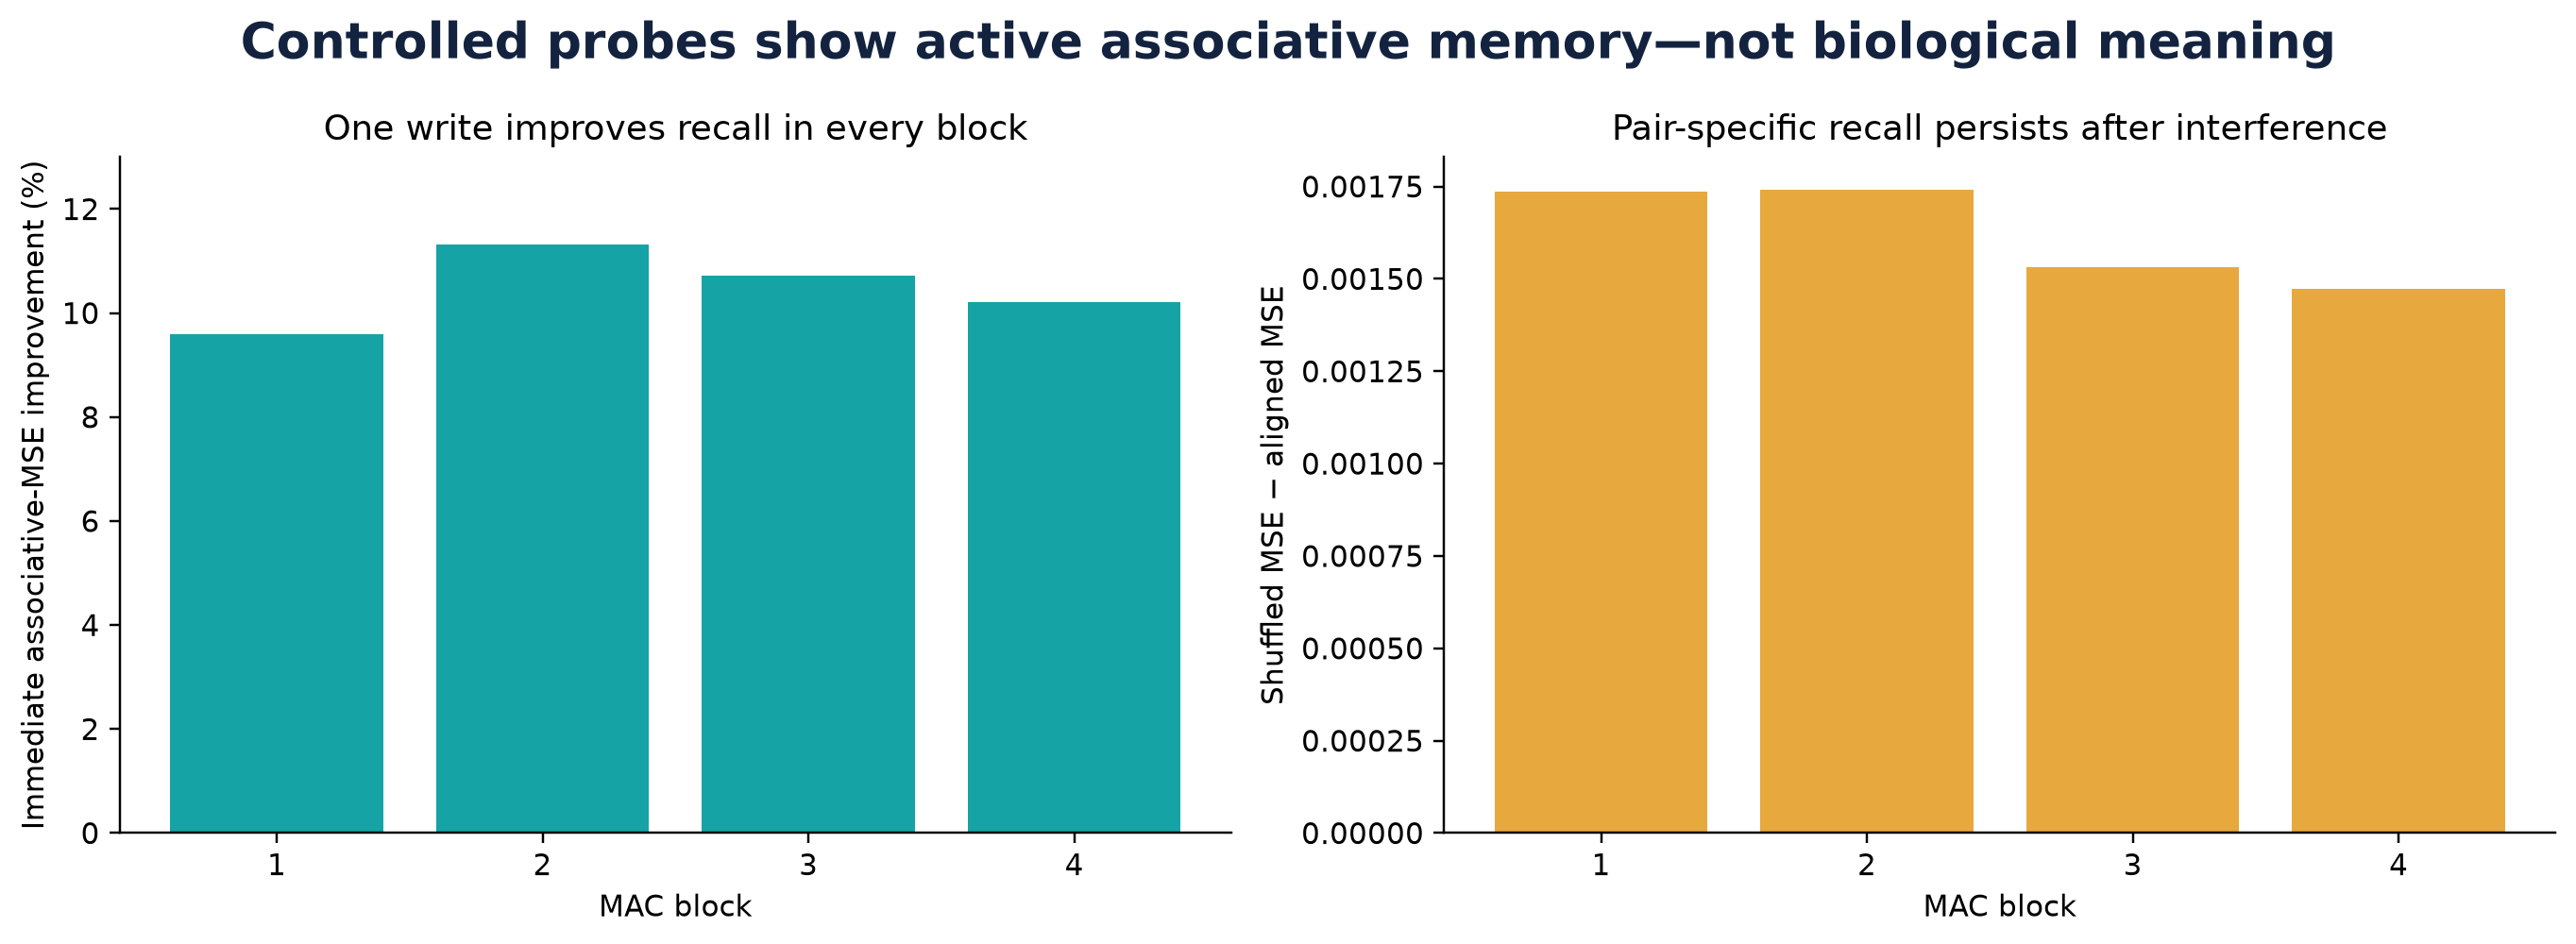
\includegraphics[width=\columnwidth]{figure_5_memory_probe.png}
\caption{Controlled neural-memory probe. Every block reduced the predefined association loss after an adaptive write.}
\label{fig:probe}
\end{figure}

\subsection*{Decoder restrictions dominated generative quality}
Hard top-$k$ truncation produced marked collapse: the strict $T=0.8,k=128,p=0.99$ policy had low aligned diversity and poor composition. Removing top-$k$ while retaining $T=0.8$ progressively restored diversity and reduced mismatch. The unrestricted $T=0.8$, no-$k$, $p=1.0$ policy was selected descriptively because it best preserved diversity and minimized 6-mer JSD among tested settings, not because it was tested on an independent selection set.

\begin{figure}[H]
\centering
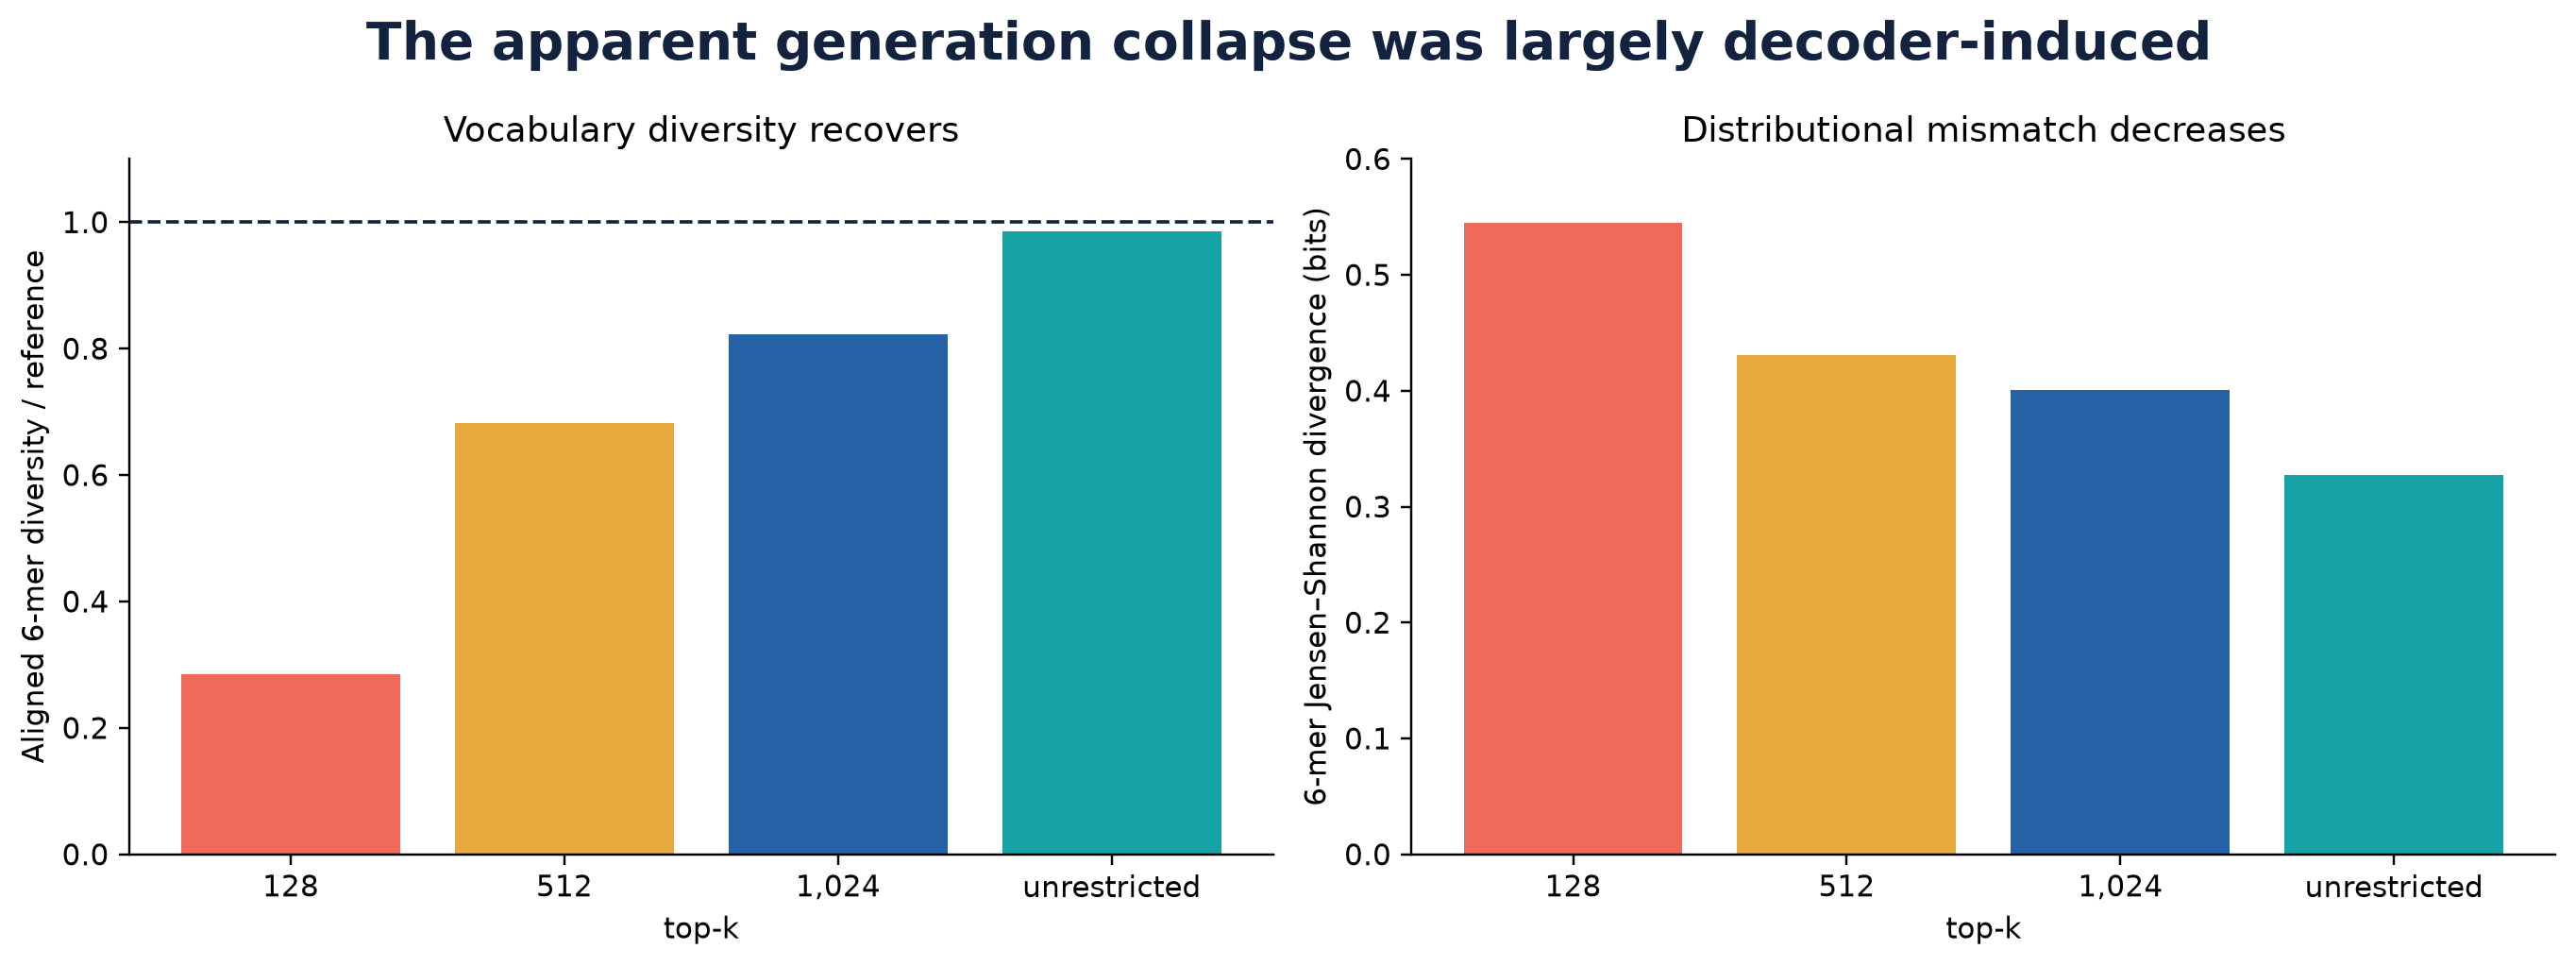
\includegraphics[width=\columnwidth]{figure_3_topk_ablation.png}
\caption{Decoding ablation. Restrictive top-$k$ sampling suppressed diversity; no-$k$ policies approached reference diversity and reduced 6-mer divergence.}
\label{fig:ablation}
\end{figure}

\begin{table*}[t]
\centering
\caption{Reference versus the descriptively best unrestricted decoding policy ($T=0.8$, no top-$k$, $p=1.0$). Ratios are generated/reference.}
\label{tab:generation}
\small
\begin{tabularx}{0.98\textwidth}{@{}XrrrX@{}}
\toprule
Metric & Reference & Generated & Ratio or difference & Interpretation\\
\midrule
GC fraction & 0.5142 & 0.4671 & $-0.0470$ & substantial AT bias\\
Nucleotide entropy (bits) & 1.9877 & 1.9955 & $+0.0079$ & near-maximal base balance; not genome realism\\
Aligned diversity & 0.9219 & 0.9111 & 0.988 & close to reference\\
Overlapping diversity & 0.6384 & 0.6572 & 1.029 & close, slightly higher\\
Median ORF count & 28.0 & 37.5 & 1.339 & many calls, but shorter structures\\
Longest ORF (bp) & 864 & 372 & 0.431 & deficient long coding structure\\
Gene calls per 10 kb & 8.138 & 8.138 & 1.000 & matched median; small sample\\
Predicted coding density & 0.494 & 0.330 & 0.668 & under-organized coding sequence\\
Median predicted gene length (bp) & 504 & 345 & 0.685 & shorter calls\\
Median intergenic distance (bp) & 72 & 506 & 7.03 & excessive spacing\\
6-mer JSD & 0 & 0.3261 & --- & strong high-order mismatch\\
\bottomrule
\end{tabularx}
\end{table*}

\subsection*{Local coding-like evidence appeared, but gene organization did not}
The unrestricted samples had near-reference nucleotide entropy and pairwise diversity, and Prodigal produced the same median number of CDS calls per 10 kb as in the matched reference fragments. Together with the presence of six-frame ORFs, this indicates that the sampled conditional distribution contains enough local codon, frame and initiation/termination evidence to trigger a prokaryotic gene model; it argues against complete motif or vocabulary collapse. It does not show that c16 formed an explicit ``gene representation,'' because Prodigal evaluated decoded DNA rather than hidden or memory states.

The arrangement and persistence of those signals remained deficient. GC content was 4.70 percentage points low, the longest heuristic ORFs were less than half as long, predicted coding density was 0.330 rather than 0.494, median Prodigal calls were 32\% shorter, and median gaps between calls were seven times longer. Divergence increased with $q$ and reached 0.326 at $q=6$. The model therefore reproduced some local coding-like cues but did not sustain them into reference-like gene length, coding occupancy or compact bacterial gene organization.

\begin{figure}[H]
\centering
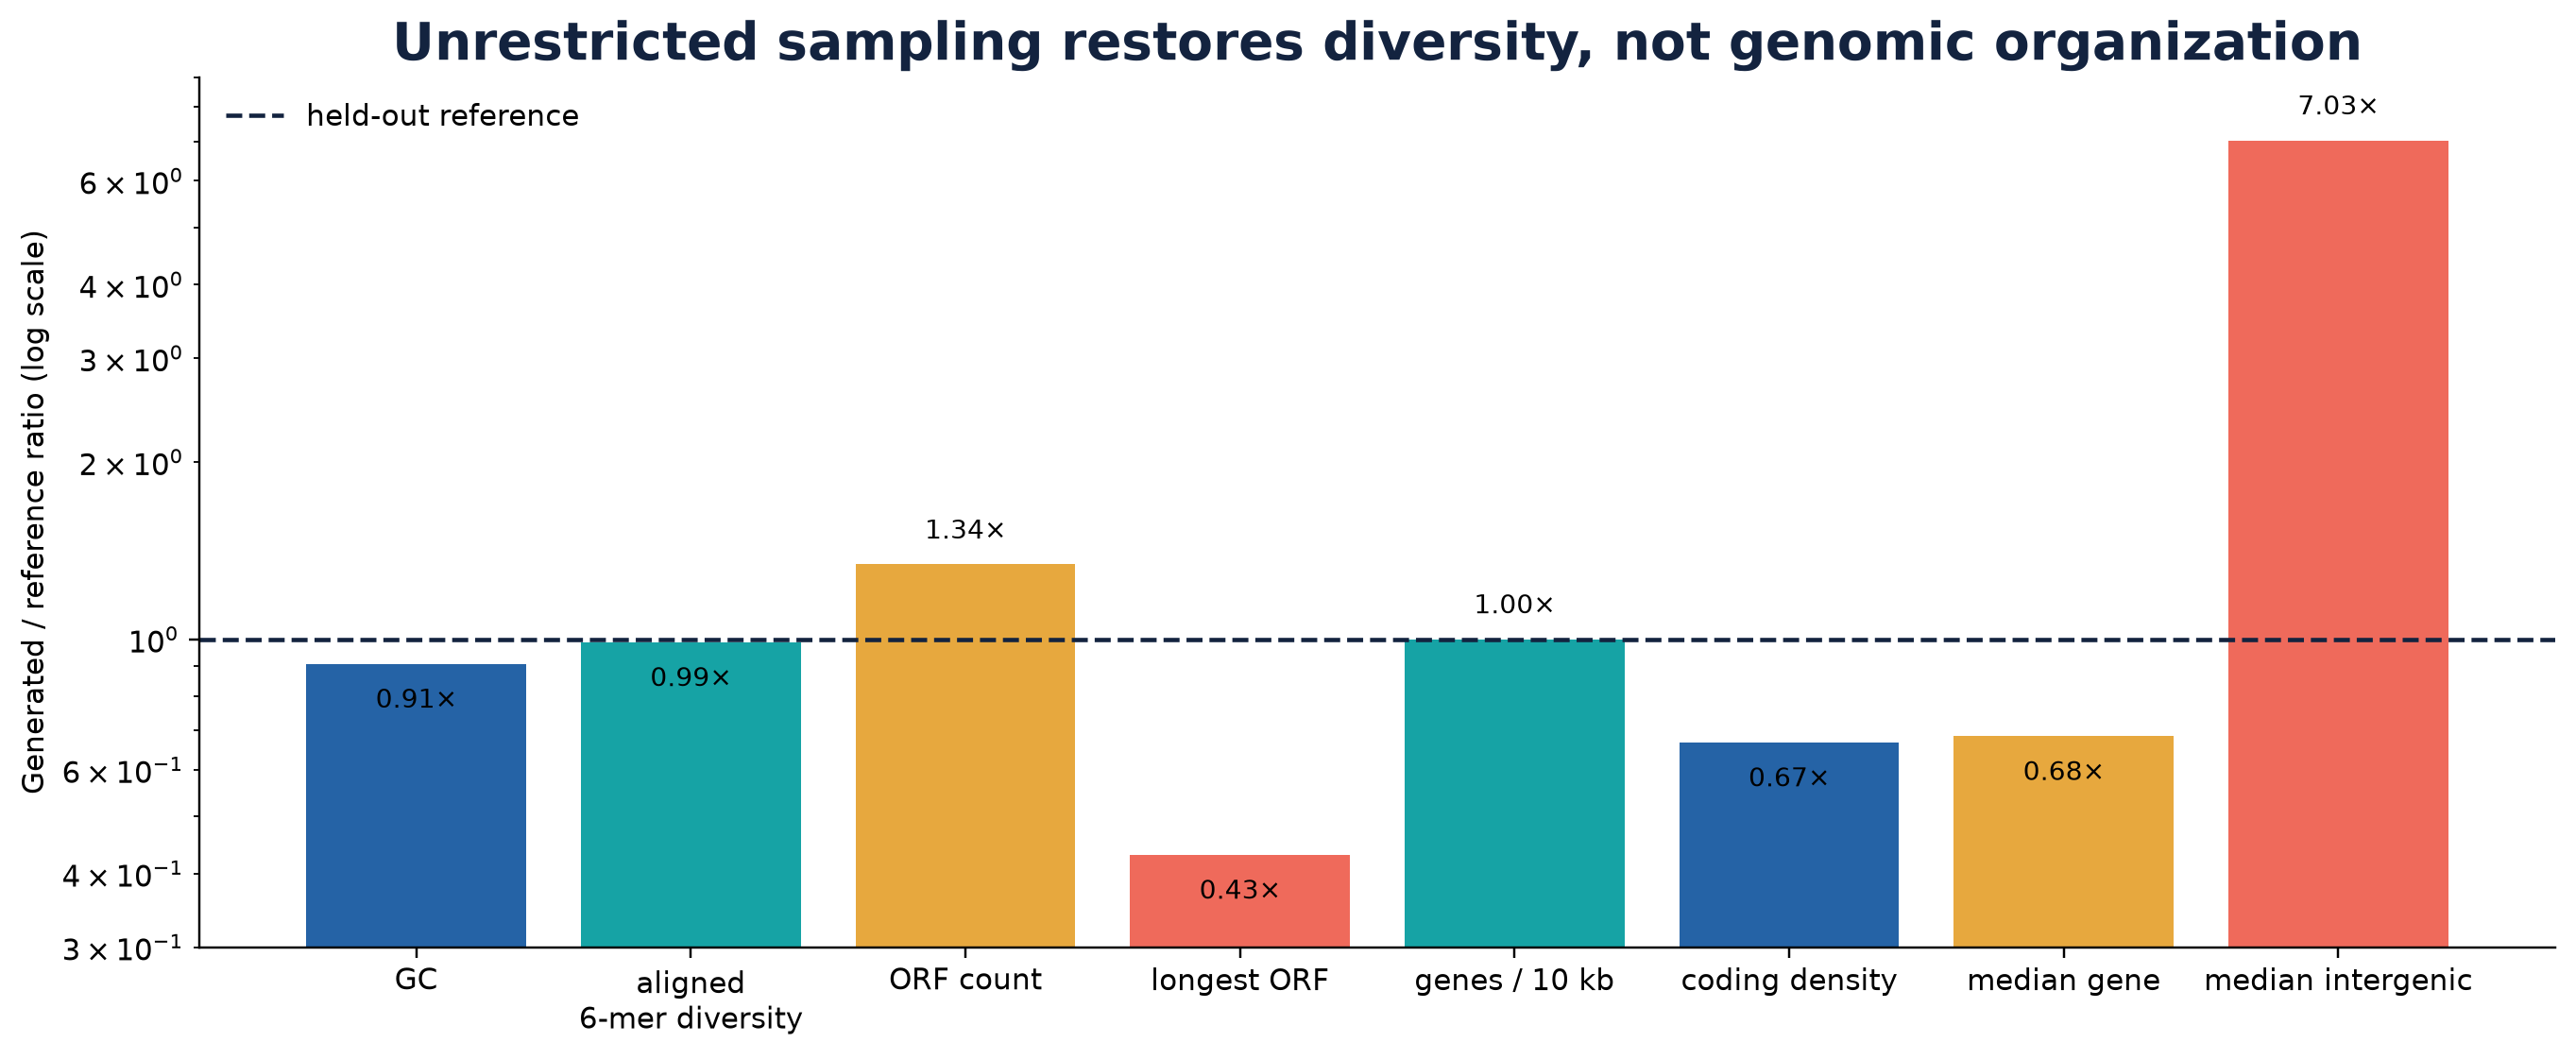
\includegraphics[width=\columnwidth]{figure_4_biological_calibration.png}
\caption{Biological calibration for the unrestricted decoder. Matching a gene-call rate coexisted with low GC, short predicted genes and excessive intergenic spacing.}
\label{fig:bio}
\end{figure}

\subsection*{PCA was diagnostic, not taxonomic evidence}
Memory PCA covered 206 segments from eight streams but only accession \code{GCA\_000249155.2}. PC1 and PC2 explained 39.1\% and 17.4\% of variance. PC1 correlated weakly with GC fraction ($r=0.079$) but strongly with normalized stream position ($r=0.683$), suggesting that the dominant exported memory trajectory may track sequence progression or state drift. The bounded trace had mean BPB 1.9965, mean memory-update norm 1.456 and mean surprise norm 0.0443; these summarize the trace subset and should not replace the main validation BPB.

Embedding PCA used eight stream means, again all from the same accession and labelled \textit{E. coli}. PC1 and PC2 explained 58.6\% and 23.9\%. Because there is no between-species or between-ANI variation, colouring these points by taxonomy cannot test taxonomic separation. The analysis validates the extraction and plotting pipeline only.

\begin{figure*}[t]
\centering
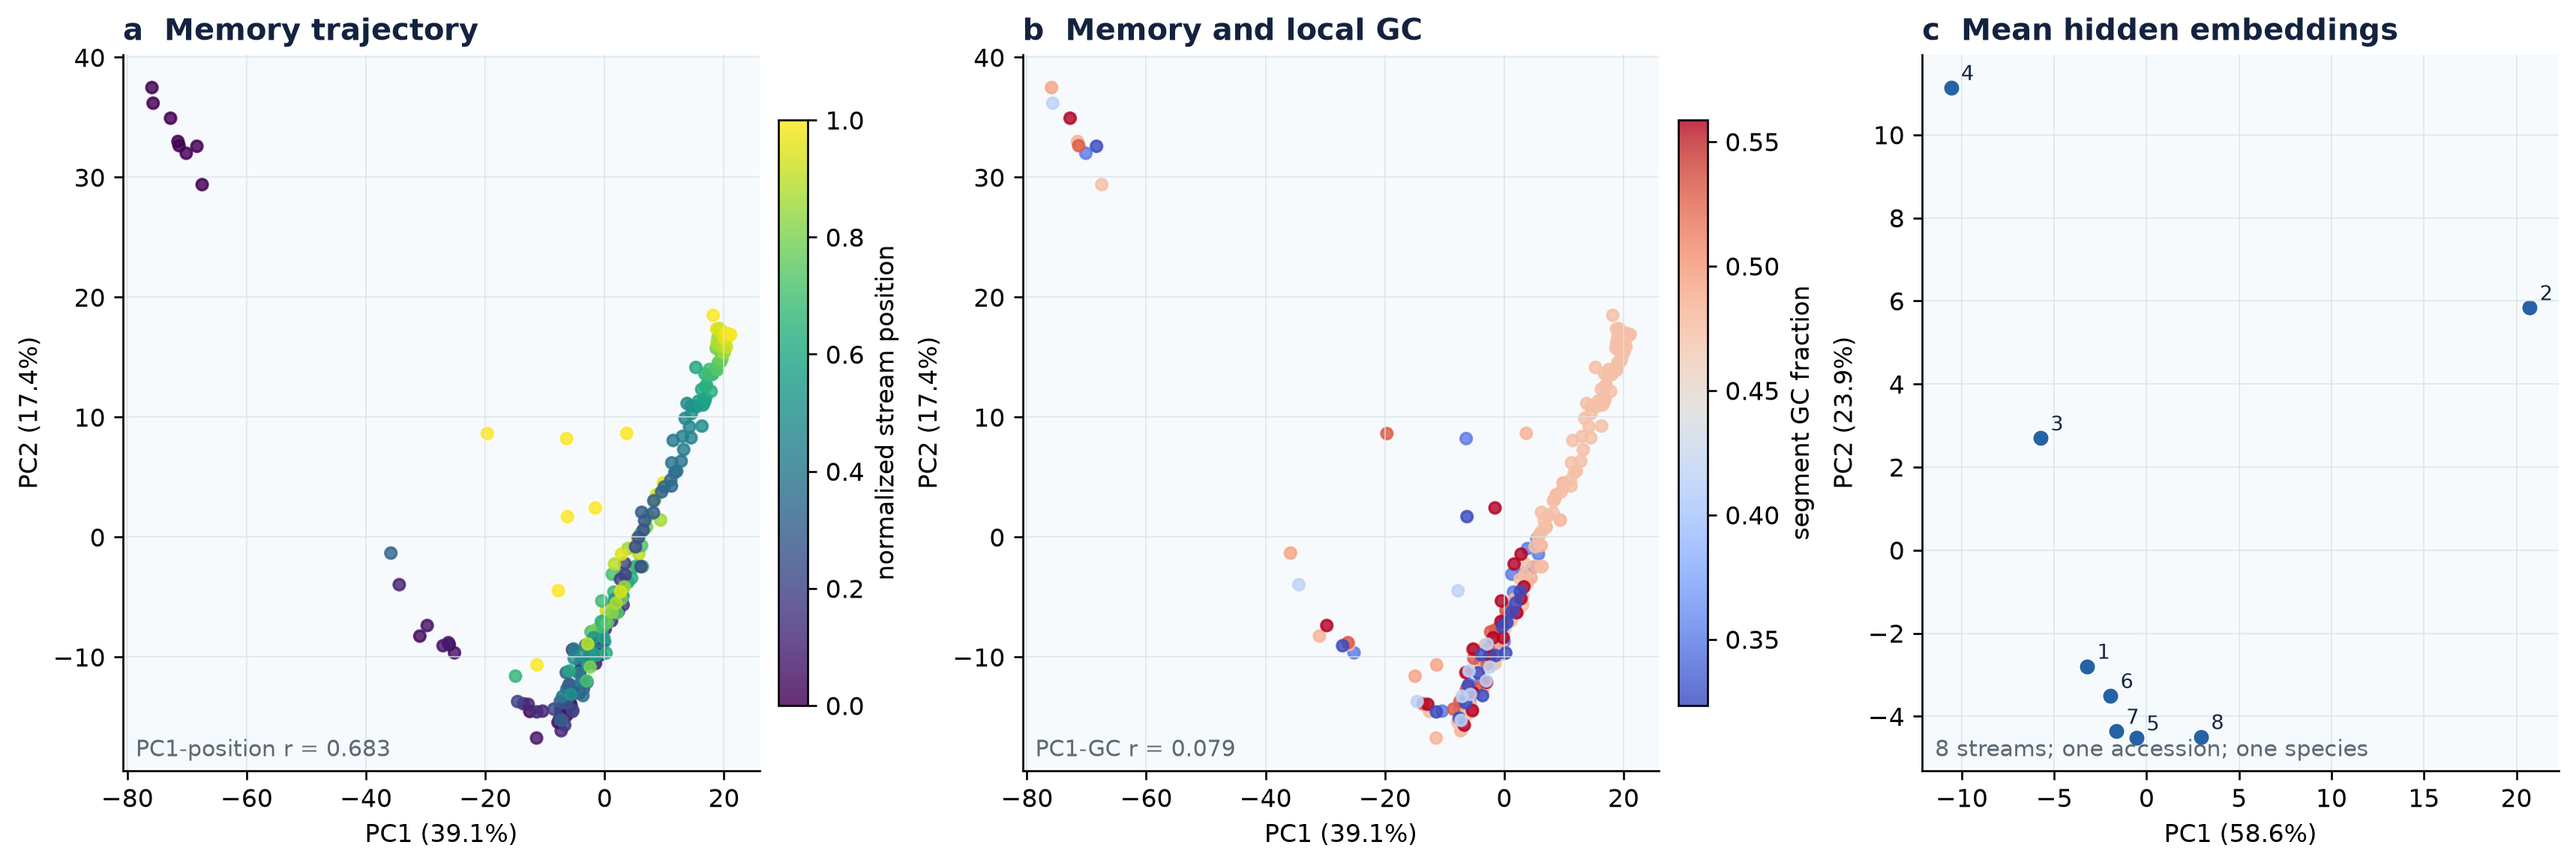
\includegraphics[width=0.96\textwidth]{figure_7_pca_diagnostics.png}
\caption{\textbf{Exploratory PCA diagnostics from Drive-backed c16 traces.} \textbf{a}, memory-state observations coloured by normalized stream position. \textbf{b}, the same memory projection coloured by segment GC fraction. \textbf{c}, mean hidden embeddings for eight streams. All observations derive from one accession; separation cannot be interpreted as taxonomy. Pearson $r$ values describe linear sample correlations and are not causal effects.}
\label{fig:pca}
\end{figure*}

\section*{Relationship to the Titans architecture}
Titans defines an architectural family, not one fixed model. The c16 implementation preserves its central MAC mechanism: a deep neural memory is queried before attention and updated afterwards from an associative key--value gradient, with learned surprise retention and forgetting \cite{behrouz2025titans}. It also retains the paper-default two-layer residual memory, width-4 causal projections and query/key normalization described mathematically above.

c16 adapts this mechanism to DNA and available compute. It uses the specified 6-mer vocabulary and compact dimensions, an explicit leakage-safe $[P;H;Z]$ mask, exact sequential writes within each 32-token segment and a three-segment outer-gradient horizon. Independent streams have independent fast states. The associative loss includes a factor $1/2$ relative to the paper; this leaves its optimum unchanged but halves the inner gradient at a fixed state. Accordingly, c16 is paper-traceable rather than a bit-for-bit reproduction of an unspecified reference model.

Equation-level float64 oracles, backend parity, future-token perturbations, stream-isolation tests and checkpoint-resume tests verify the declared implementation contracts. They establish mathematical and causal consistency, not improved BPB or biological meaning. Detailed mappings and test evidence are provided in Supporting Information Tables~\ref{tab:mapping} and~\ref{tab:verification}.

\section*{Interpretation and limitations}
Three conclusions are supported. First, the training and resume path produced a finite compact model with a modest held-out signal. Second, the neural memory is not inert: it updates, retrieves, and improves a controlled association objective in every block. Third, unrestricted decoding produces diverse DNA with several local genetic-looking statistics, whereas strong top-$k$ filters can obscure that capability.

Several stronger conclusions are not supported. The study does not show that adaptive memory improves held-out prediction because no matched 5-million-base no-memory and frozen-memory controls were evaluated. It does not show taxonomic representation because the PCA trace contains one accession. Prodigal output does not establish promoters, expressed genes, functional proteins, genome coherence or viability, and it cannot localize coding-like information to a hidden layer or to neural memory. Similar entropy and gene-call rate can arise while high-order sequence organization is wrong, as the 6-mer JSD, coding-density and intergenic results demonstrate. The exact 5-million-base training trajectory also lacks an exported taxonomic exposure table, so it cannot be treated as a representative sample of the nominal 15-Gbp parent corpus. The small number and length of generations make medians unstable; no confidence intervals were computed for the tabled biological diagnostics. Finally, decoder selection and evaluation used the same ablation, so the preferred policy is exploratory.

The results are promising specifically because the failure mode is structured rather than complete collapse: diversity is recoverable by decoding, the association machinery works, and several local statistics are present. Yet incomplete genome organization is the dominant result. Scaling parameter count without broadening whole-genome exposure, controlling the architecture comparison and strengthening evaluation could simply produce a larger model with the same bias.

\begin{figure}[H]
\centering
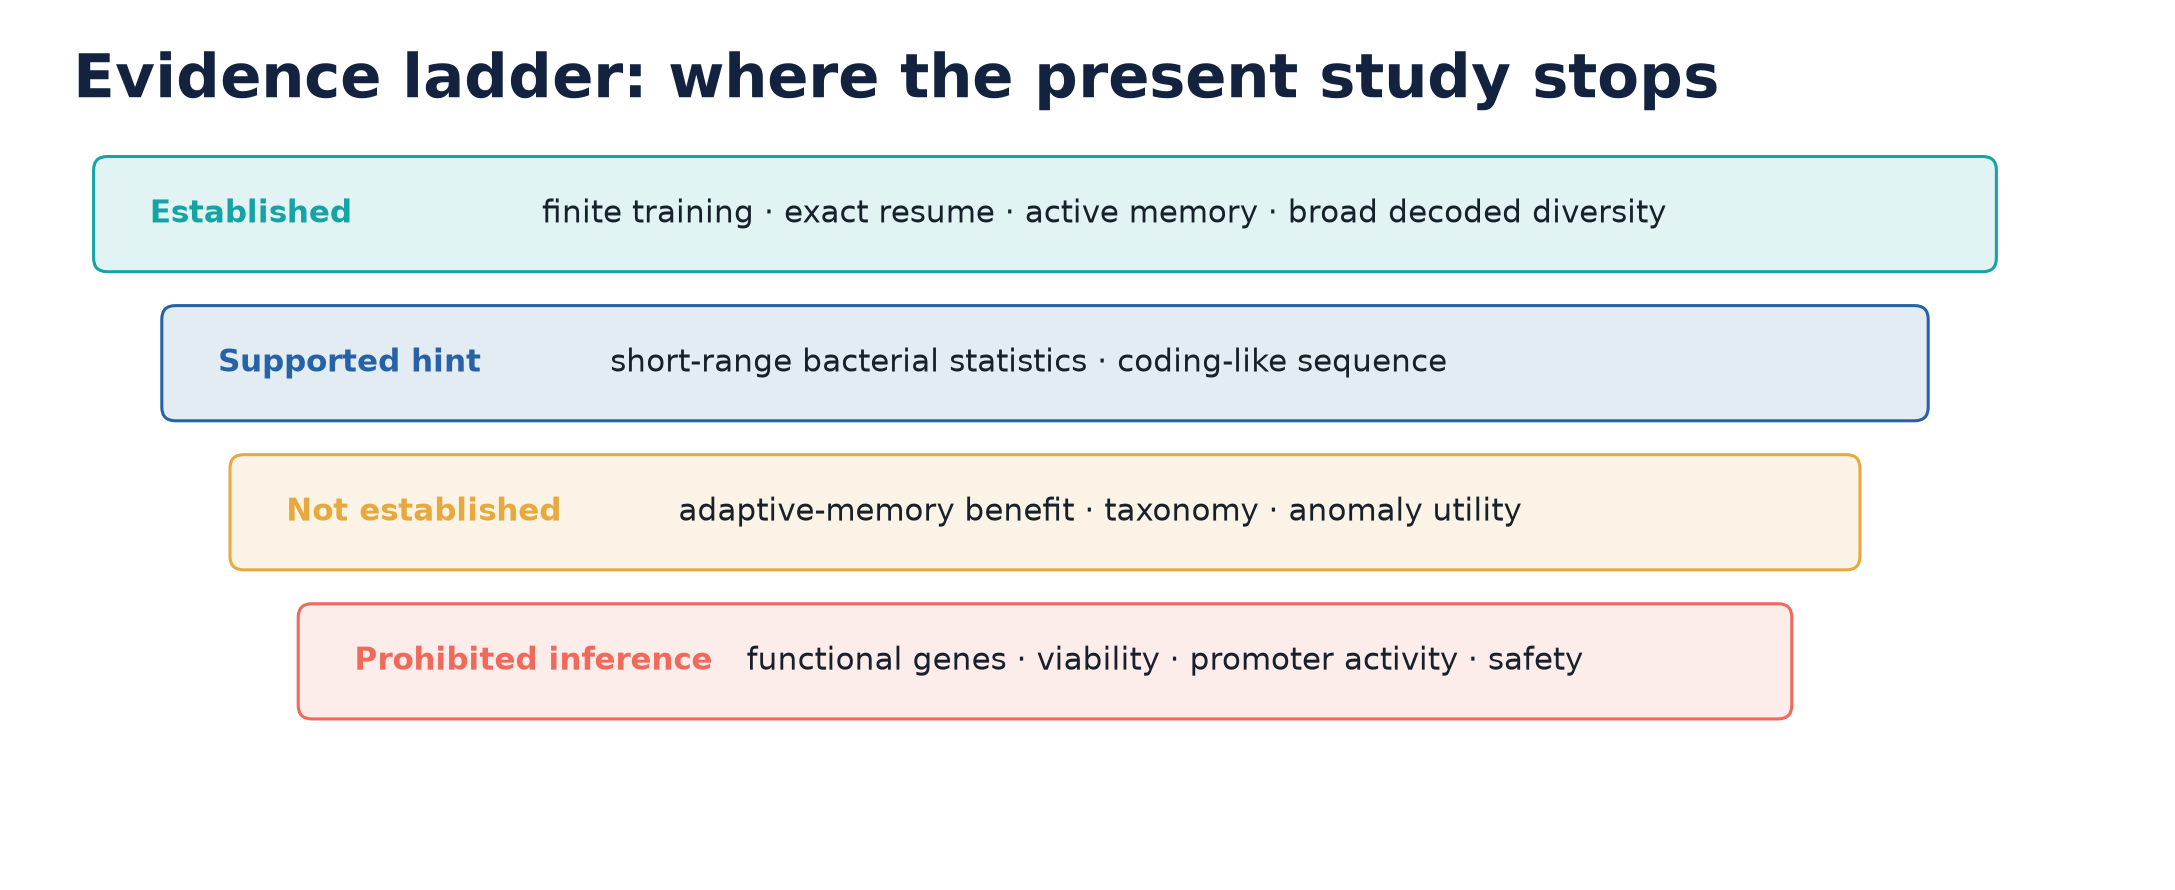
\includegraphics[width=\columnwidth]{figure_6_evidence_ladder.png}
\caption{Evidence ladder. Current results support learning and mechanism activity, but stop below comparative memory benefit and biological function.}
\label{fig:evidence}
\end{figure}

\section*{Recommended next study}
The next experiment should preserve entire genomes within nested ANI-aware training panels while increasing diversity in controlled stages. A practical progression is: (1) freeze non-overlapping training, validation and test accessions; (2) train adaptive memory first on a whole-genome \textit{E. coli} panel and evaluate held-out BPB, finite-state telemetry, generation and PCA; (3) only after a predefined adaptive gate is met, train a compute- and data-matched no-memory control; (4) if adaptive memory beats that control with paired accession/clade bootstrap uncertainty, add frozen-memory, repaired shallow-memory and second-seed replication; and (5) broaden to distinct \textit{Escherichia} and related clades for genuine taxonomy-coloured representation tests.

Generation evaluation should use a decoder policy frozen before test analysis, substantially more samples, independent prompts and chromosome-scale diagnostics. Report confidence intervals for GC, $q$-mer JSD, ORF statistics and coding organization. Probe memory with delayed association, stream resets, shuffled controls and matched local/GC baselines. Anomaly detection should be assessed on held-out synthetic perturbations and natural-region benchmarks at a fixed false-positive rate; generative plausibility alone cannot validate anomaly utility.

\section*{Notation summary}
\begin{table}[H]
\centering
\caption*{Symbols used in the mathematical specification.}
\small
\begin{tabularx}{\columnwidth}{@{}lX@{}}
\toprule
Symbol & Meaning\\
\midrule
$a_t,t,a_{<t}$ & token at global position $t$, its index, and preceding tokens\\
$V,E,x_t$ & vocabulary size, embedding matrix and token embedding\\
$d,C,n,i$ & model width, segment length, segment index and within-segment index\\
$p,P$ & number and matrix of persistent tokens\\
$z,y,q,k,v,h$ & block input/output, read query, write key/value and retrieval\\
$W_Q,W_K,W_V$ & learned query/key/value projection matrices\\
$\mathcal C_Q,\mathcal C_K,\mathcal C_V$ & causal width-4 depth-wise convolutions\\
$M_\phi,\phi,\phi_r$ & memory function, all fast parameters and tensor $r$\\
$W_i,b_i,W_o,b_o$ & memory MLP expansion/output weights and biases\\
$\ell,g$ & associative loss and its fast-parameter gradient\\
$S,\eta,\theta,\alpha$ & surprise momentum, retention, write scale and forgetting fraction\\
$\omega,\mathcal L_{\rm LM}$ & slow parameters and language-model loss\\
$\mathcal T,N_b$ & valid target positions and represented valid bases\\
$r_j,T,\mathcal A,\pi_j$ & logit, temperature, allowed candidates and sample probability\\
$P_q,Q_q,R_q$ & reference, generated and mixture $q$-mer distributions\\
$X,n_s,d_f,u_r,c_{j,r}$ & PCA matrix, counts/dimension, loading and score\\
$\R,\norm{\cdot}_2,\had$ & real space, Euclidean norm and element-wise product\\
\bottomrule
\end{tabularx}
\end{table}

\section*{Reproducibility and provenance}
The manuscript is compiled from source-controlled LaTeX and frozen numerical inputs. The evaluated checkpoint SHA-256 begins \code{21898362} and ends \code{4541}; the complete digest is recorded in the build manifest. The run ledger records training, generation and decoding-ablation events. Drive-exported PCA JSON files are retained beside the manuscript source and hashed in the build manifest. The article deliberately distinguishes the 1.9828-BPB main validation result from the 1.9965-BPB bounded memory-trace subset.

\section*{Data and code availability}
Code, the frozen study protocol, notebook workflows and this article source reside in the SeqTrainer repository. Large checkpoints and run artifacts remain in the Drive-backed study root. Access to biological source data should follow the original dataset licences and accession metadata.

\section*{Acknowledgement of scope}
This document is a journal-style exploratory report generated before confirmatory controls. It should not be represented as peer-reviewed evidence or as validation of synthetic biological function or safety.

\begin{thebibliography}{9}
\bibitem{behrouz2025titans}
A. Behrouz, P. Zhong and V. Mirrokni. Titans: Learning to memorize at test time. \emph{Advances in Neural Information Processing Systems} (2025). \href{https://proceedings.neurips.cc/paper_files/paper/2025/file/a4ca07aa108036f80cbb5b82285fd4b1-Paper-Conference.pdf}{Official paper PDF}.

\bibitem{vaswani2017attention}
A. Vaswani \emph{et al.} Attention is all you need. \emph{Advances in Neural Information Processing Systems} \textbf{30} (2017).

\bibitem{hornik1989multilayer}
K. Hornik, M. Stinchcombe and H. White. Multilayer feedforward networks are universal approximators. \emph{Neural Networks} \textbf{2}, 359--366 (1989).

\bibitem{hyatt2010prodigal}
D. Hyatt \emph{et al.} Prodigal: prokaryotic gene recognition and translation initiation site identification. \emph{BMC Bioinformatics} \textbf{11}, 119 (2010).

\bibitem{shaw2023skani}
J. Shaw and Y. W. Yu. Fast and robust metagenomic sequence comparison through sparse chaining with skani. \emph{Nature Methods} \textbf{20}, 1661--1665 (2023).

\bibitem{gtdbr220}
Genome Taxonomy Database. GTDB release R220 statistics: 596,859 genomes in 113,104 species clusters (24 April 2024). \url{https://gtdb.ecogenomic.org/stats/r220}.
\end{thebibliography}

\section*{Supporting Information}
The following tables document architectural correspondence and verification without interrupting the main results narrative. ``Maintained'' denotes agreement with a declared mechanism, not identical data, scale or software to the Titans experiments.

\begin{table*}[!t]
\centering
\caption{Detailed correspondence between the Titans architecture and the evaluated c16 implementation. Titans is an architectural family rather than one fixed parameterization; the second column therefore distinguishes equations and defaults described in the paper from choices required for this executable model.}
\label{tab:mapping}
\scriptsize
\setlength{\tabcolsep}{3pt}
\renewcommand{\arraystretch}{1.12}
\begin{tabularx}{\textwidth}{@{}>{\raggedright\arraybackslash}p{0.13\textwidth}>{\raggedright\arraybackslash}p{0.235\textwidth}>{\raggedright\arraybackslash}p{0.29\textwidth}>{\raggedright\arraybackslash}X@{}}
\toprule
Component & Titans paper / reference formulation & Evaluated c16 implementation & Motivation and implication\\
\midrule
Architecture family & Titans presents several neural-memory arrangements, including Memory as Context (MAC). & Selects MAC and stacks four blocks; each block retrieves neural memory, performs causal attention and then publishes an updated fast state. & Isolates the mechanism under study. Results apply to this compact MAC realization, not every Titans variant.\\
Input and objective & General sequence modelling with token representations and an outer autoregressive objective. & Non-overlapping 6-mers; $V=4{,}103$; learned token and 32-position embeddings; tied input/output embeddings; next-6-mer likelihood reported as BPB. & Adapts the model to DNA and makes information rate comparable per nucleotide. Six-mer tokenization limits resolution and does not encode biological annotation.\\
Model scale & The paper studies a family of widths, depths and memory configurations rather than one mandatory size. & $d=128$, four MAC blocks, four attention heads, four persistent tokens per block and approximately 2.52 million slow parameters. & Fits T4-scale exploratory training. It is a compact feasibility model, not a scale-matched reproduction of the paper's largest experiments.\\
Neural-memory function & Associative memory may be a deep MLP; the paper motivates at least two layers and uses a residual deep-memory form. & $M_{\phi}(u)=u+\operatorname{LN}[W_o\operatorname{GELU}(W_i u+b_i)+b_o]$, with $128\rightarrow512\rightarrow128$ affine maps. All affine and layer-normalization parameters are fast state. & Preserves the paper-default two-layer, four-times-expanded nonlinear memory. ``Depth two'' refers to the two affine memory layers, not the separate key/value projections.\\
Q/K/V construction & Learned query, key and value projections; the paper implementation uses short causal convolution and Q/K normalization. & Independent bias-free linear Q/K/V maps followed by separate causal depth-wise width-4 convolutions; Q and K are L2-normalized, V is not. Three preceding raw inputs are retained per stream across segment boundaries. & Maintains the declared projection policy without resetting convolution at a segment boundary. Normalization changes key/query scale, not the associative target value.\\
Associative loss & Printed as $\norm{M_{\phi}(k)-v}_2^2$. & $\ell=\tfrac12\norm{M_{\phi}(k)-v}_2^2$, summed over 128 output channels; $g=\nabla_{\phi}\ell$ is computed with higher-order autograd. & The minimizers are unchanged, but $g$ is exactly half the paper-printed gradient at fixed $(\phi,k,v)$. Write magnitude must therefore be interpreted jointly with learned $\theta$; \code{paper\_exact} is not prefactor identity.\\
Surprise momentum & $S_t=\eta_t\had S_{t-1}-\theta_t\had\nabla\ell_t$. Past surprise and momentary gradient surprise are combined before writing. & Implements the same recurrence independently for every fast-parameter tensor; telemetry separately records retained past surprise, momentary surprise, their cosine and combined RMS. & Preserves the sign and momentum mathematics while making the two contributions observable for diagnosis. Telemetry does not alter the update.\\
Forgetting & $M_t=(1-\alpha_t)\had M_{t-1}+S_t$, where $\alpha_t$ is the removed fraction. & Applies the equation to every fast tensor. Learned sigmoid gates initialize at $\alpha=0.001$, $\eta=0.9$ and $\theta=0.001$. & Retains 99.9\% of each old fast weight before adding surprise at initialization; avoids the incomparable legacy shallow initialization. Gates remain trainable.\\
Gate granularity & The recurrence is data-dependent; the paper equations do not uniquely determine every tensor-broadcasting choice. & Separate gate heads for memory input and output layers emit $\alpha,\eta,\theta$ by output channel; vectors broadcast over each neuron's incoming dimension and cover affine biases plus LN scale/bias. & Allows different memory layers and channels to learn different timescales while keeping the contract inspectable. This is an explicit implementation choice.\\
Read/write timing & MAC supplies memory retrieval as attention context; the paper also develops chunkwise parallel approximations for efficient training. & For segment $n$, all 32 retrievals use incoming $\phi_{n,0}$. Attention consumes $[P;H_n;Z_n]$; only afterwards do 32 exact sequential writes produce $\phi_{n,32}$. & Prevents an updated memory from leaking information into earlier outputs. It also means c16 does not retrieve its own within-segment writes until the next segment.\\
Causal integration & Context must respect autoregressive ordering. & A boolean block-causal mask lets position $i$ attend to all persistent tokens and retrieval/input prefixes $1{:}i$, never $j>i$; attention output has residual addition and layer normalization. & Makes the no-future-information contract explicit and perturbation-testable. The $[P;H;Z]$ packing order is c16-specific.\\
State scope and reach & Neural memory is updated online along a sequence and trained through the outer objective. & Each logical stream and each block owns independent $(\phi,S,Q\text{-history},KV\text{-history})$. Numerical state persists along contiguous segments; the outer autograd graph is detached every three segments (96 tokens, at most 576 represented bases). & Prevents cross-accession contamination and bounds memory use. Long-lived numerical memory is retained, but slow-parameter credit assignment cannot cross the truncation boundary.\\
Numerical policy & The paper motivates scalable memory updates and efficient approximations. & \code{paper\_exact}: exact sequential nonlinear fast-weight gradients, no surprise-norm cap, no RMS conditioning, $\theta_{\max}=1$; FP32 activations and reviewed exact-accelerated memory/math-SDPA path. & Maximizes equation traceability for c16 at higher compute cost. The separately declared stabilized and legacy norm-4 policies were not active in this checkpoint.\\
Training exposure & Paper experiments use task-specific corpora, schedules and scales. & Adaptive-memory-only exploratory run; seed 20260741; batch size 1; learning rate $3\times10^{-5}$; outer gradient clip 0.5; 5 million valid training bases. & Tests whether the implementation merits scale-up. Without a matched 5M no-memory/frozen control or second seed, it cannot establish an adaptive-memory advantage.\\
\bottomrule
\end{tabularx}
\end{table*}

\begin{table*}[!t]
\centering
\caption{Verification and evidence matrix for the c16 paper-to-code contract. Numerical oracles test implementation properties; run artifacts test execution and provenance. Neither evidence class alone establishes predictive benefit from adaptive memory or biological function.}
\label{tab:verification}
\scriptsize
\setlength{\tabcolsep}{3pt}
\renewcommand{\arraystretch}{1.12}
\begin{tabularx}{\textwidth}{@{}>{\raggedright\arraybackslash}p{0.17\textwidth}>{\raggedright\arraybackslash}p{0.35\textwidth}>{\centering\arraybackslash}p{0.08\textwidth}>{\raggedright\arraybackslash}X@{}}
\toprule
Contract & Evidence exercised & Result & Interpretation and remaining boundary\\
\midrule
Residual memory & FP64 oracle compares \code{PaperResidualMemory} against $u+\operatorname{LN}[W_o\operatorname{GELU}(W_i u+b_i)+b_o]$ and checks the $4d$ hidden width. & Pass & Confirms the implemented function and dimensions, not that depth improves prediction.\\
Associative objective & Sum/mean reduction oracle verifies $\ell_{\mathrm{mean}}=\ell_{\mathrm{sum}}/d$; direct differentiation exercises all fast tensors. & Pass & Fixes reduction semantics. The separate factor-$1/2$ convention remains a documented difference from the printed paper objective.\\
Recurrence and gates & Hand-calculated and paper-deep FP64 tests compare every fast tensor with $S_t=\eta_tS_{t-1}-\theta_tg_t$ and $\phi_t=(1-\alpha_t)\phi_{t-1}+S_t$ to absolute tolerance $10^{-12}$. & Pass & Confirms signs, broadcasting, initialized channel gates and update order for tested cases; it does not prove long-run stability by itself.\\
Projection history & Width-4 causal-convolution oracle compares two consecutive segments against a single explicitly padded sequence; Q/K normalization is checked after projection. & Pass & Shows segment boundaries preserve the preceding three projection inputs and introduce no reset artifact in the tested path.\\
Read snapshot and commit & Segment-shape/read-snapshot tests verify that all retrievals use the incoming state, padded tail positions do not write, and one replacement state is published after the segment. & Pass & Confirms c16's declared pre-read/post-write semantics; these semantics remain an implementation choice within MAC.\\
Attention causality & Exhaustive boolean-mask complement test plus future-retrieval and future-token perturbations compare all earlier outputs/logits. & Pass & Supports the no-future-leakage contract for the tested mask and attention adapters; it is not a dataset-isolation test.\\
Backend equivalence & Reference-versus-exact-accelerated suites compare sequence output, retrieval, fast weights, surprise, input gradients and parameter gradients in float64 and float32; SDPA is compared with reference attention forward/backward. & Pass & Supports use of the accelerated training path without a known mathematical substitution within tested tolerances. It does not cover arbitrary hardware/library versions.\\
Higher-order learning & Thirty-two-update gate-gradient test, three-segment finite-gradient test and trainer horizon test exercise backward-through-update and detachment at the configured boundary. & Pass & Shows slow parameters and gate heads can receive meta-gradients through the declared horizon; it does not show useful credit assignment beyond three segments.\\
Stream isolation and controls & Batched-versus-isolated stream test, stream-local reset/serialization test and explicit adaptive, frozen and no-memory mode checks. & Pass & Rules out tested cross-stream state sharing and verifies control semantics. It does not substitute for training matched controls.\\
Finite guards & Multi-step CPU training test plus injected non-finite test verify finite updates and identification of the first failing tensor/step. The completed c16 training and trace contain finite state telemetry. & Pass & Detects numerical failure and documents this run's stability; absence of non-finites does not imply optimal conditioning or convergence.\\
Checkpoint/resume & Checkpoint oracle restores model, optimizer, scheduler, data cursor, RNG and complete per-block fast state; the c16 resume artifact records a successful reload path. & Pass & Supports continuation consistency for the tested artifact and software path; it is not proof of bitwise reproducibility across platforms.\\
Configuration lock & \code{StageCModelConfig} and protocol validation require depth 2, expansion 4, kernel 4, normalized Q/K, per-layer channel gates and, for \code{paper\_exact}, summed loss with no cap or RMS conditioning. & Pass & Prevents silent policy drift at construction and run launch. Correctly declared settings can still encode a scientifically weak design.\\
Run provenance & Frozen protocol plus dated amendment bind run ID, seed, dataset/tokenizer fingerprints, command, checkpoint digest and output artifacts in the append-only study ledger. & Present & Makes c16 auditable and preserves deviations. Provenance strengthens traceability, not causal evidence.\\
Mechanism activity & Held-out trace reports non-zero retrieval/update/surprise statistics; controlled association probes reduce reconstruction error by 9.60--11.31\% across four blocks. & Observed & Shows the memory is active and can improve its own associative target. Only matched predictive controls can determine whether it improves BPB.\\
\bottomrule
\end{tabularx}
\end{table*}

\end{document}
